\section{测度的分解}
\label{sec:dens-decomposition}

绝对连续与相互奇异是两个极端：前者不在参考测度的零测集上放任何质量，后者把全部质量放在某个参考零测集上。一般的测度介于两者之间，例如长度加上一个点质量。本节先证明，相对于给定的参考测度，$\sigma$有限测度都能唯一地拆成这两种极端之和，并用Radon–Nikodym定理表示其中绝对连续的一份。然后在实轴上以Lebesgue测度为参考，把奇异的一份再分成点质量与没有点质量的奇异质量，并说明累积函数的普通导数只能读出其中哪一部分。

\subsection{Lebesgue分解}
\label{sec:dens-lebesgue-decomposition}

给定参考测度$\mu$与目标测度$\nu$，我们希望把$\nu$的质量分成两份：一份完全落在某个$\mu$零测集上，是$\mu$“看不见”的质量；另一份在$\mu$零测集上没有任何质量。分解有三个问题需要分别回答：两份质量怎样构造，分法是否唯一，以及看得见的那份能否写成密度。

\begin{theorem}[Lebesgue分解]
\label{thm:dens-lebesgue-decomposition}
设$\mu,\nu$是可测空间$(X,\mathcal A)$上的$\sigma$有限非负测度。则存在唯一的一对非负测度$\nu_{\mathrm{ac}},\nu_{\mathrm s}$，使
\[
\nu=\nu_{\mathrm{ac}}+\nu_{\mathrm s},\qquad\nu_{\mathrm{ac}}\ll\mu,\qquad\nu_{\mathrm s}\perp\mu .
\]
更具体地，存在$N\in\mathcal A$使$\mu(N)=0$，$\nu_{\mathrm s}(A)=\nu(A\cap N)$，$\nu_{\mathrm{ac}}(A)=\nu(A\setminus N)$。并且存在可测函数$h:X\to[0,+\infty)$，使
\begin{equation}
\nu(A)=\int_Ah\,\mathrm d\mu+\nu_{\mathrm s}(A),\qquad A\in\mathcal A ,
\label{eq:dens-lebesgue-form}
\end{equation}
$h$在$\mu$几乎处处意义下唯一。特别地，$\nu$相对于$\mu$有密度，当且仅当$\nu_{\mathrm s}=0$。
\end{theorem}

这一分解称为$\nu$相对于$\mu$的\term{Lebesgue分解}（Lebesgue decomposition），$\nu_{\mathrm{ac}}$与$\nu_{\mathrm s}$分别称为绝对连续部分与奇异部分。分解依赖参考测度。在实轴上取$\nu=\lambda|_{[0,1]}+\delta_2$。以$\lambda$为参考，$N=\{2\}$是$\lambda$零测集并承载点质量，于是$\nu_{\mathrm s}=\delta_2$，$\nu_{\mathrm{ac}}=\lambda|_{[0,1]}$。以$\delta_2$为参考，$\mathbb R\setminus\{2\}$是$\delta_2$零测集，角色互换：$\nu_{\mathrm s}=\lambda|_{[0,1]}$，$\nu_{\mathrm{ac}}=\delta_2$。

\paragraph{构造：承载最多质量的零测集}
定理中的$N$应当在保持$\mu(N)=0$的同时尽可能多地装下$\nu$的质量。若某个$\mu$零测集在$N$之外还有正的$\nu$质量，就把它并进$N$。先在$\nu$有限时用上确界实现这个想法。

\begin{proof}[存在性，$\nu$有限的情形]
令$M=\sup\{\nu(A):A\in\mathcal A,\ \mu(A)=0\}\leq\nu(X)<\infty$。对每个$k$取$\mu$零测集$N_k$使$\nu(N_k)>M-1/k$，令$N=\bigcup_kN_k$。由可数次可加性$\mu(N)=0$，所以$\nu(N)\leq M$；又$\nu(N)\geq\nu(N_k)>M-1/k$，故$\nu(N)=M$。

令$\nu_{\mathrm s}(A)=\nu(A\cap N)$，$\nu_{\mathrm{ac}}(A)=\nu(A\setminus N)$，二者都是测度，和为$\nu$。由$\mu(N)=0$与$\nu_{\mathrm s}(X\setminus N)=0$得$\nu_{\mathrm s}\perp\mu$。设$\mu(A)=0$，则$N\cup(A\setminus N)$仍是$\mu$零测集，其$\nu$质量不超过$M$；两部分不交，所以$M+\nu(A\setminus N)\leq M$。$M$有限，消去得$\nu_{\mathrm{ac}}(A)=0$，即$\nu_{\mathrm{ac}}\ll\mu$。
\end{proof}

最后的消去正是需要有限性的地方：若$M=+\infty$，不等式$M+t\leq M$不能推出$t=0$。对$\sigma$有限的$\nu$，取两两不交的$X_j$覆盖$X$且$\nu(X_j)<\infty$，在每片上对有限测度$A\mapsto\nu(A\cap X_j)$作上面的构造，得到$\mu$零测集$N_j\subset X_j$；令$N=\bigcup_jN_j$，则$\mu(N)=0$。若$\mu(A)=0$，则$\nu(A\setminus N)=\sum_j\nu((A\setminus N_j)\cap X_j)=0$，每一项是相应片上已证的绝对连续性。构造只用了可数次可加性、上确界与限制测度，没有用积分。

\paragraph{唯一性}
设$\nu=\alpha+\beta=\alpha'+\beta'$，其中$\alpha,\alpha'\ll\mu$，$\beta,\beta'\perp\mu$。取$\mu$零测集$S,S'$使$\beta(X\setminus S)=0$，$\beta'(X\setminus S')=0$，令$T=S\cup S'$，则$\mu(T)=0$，$\beta,\beta'$在$X\setminus T$上都没有质量。对任意$A$，$\mu(A\cap T)=0$推出$\alpha(A\cap T)=\alpha'(A\cap T)=0$，所以$\beta(A\cap T)=\nu(A\cap T)=\beta'(A\cap T)$；又$\beta(A\setminus T)=\beta'(A\setminus T)=0$，所以$\alpha(A\setminus T)=\nu(A\setminus T)=\alpha'(A\setminus T)$。两部分相加，得$\alpha=\alpha'$，$\beta=\beta'$。

唯一性的论证只在$T$与$X\setminus T$上分别读取$\nu$，没有做减法，因此不需要任何有限性。$\sigma$有限条件只在存在性中用到，并且不能随意去掉：在$[0,1]$的Borel集上取$\mu=\lambda$，$\nu$为计数测度。若有满足要求的分解，取$N$使$\lambda(N)=0$、$\nu_{\mathrm s}([0,1]\setminus N)=0$；由于$\lambda(N)=0$，可取$x\notin N$，则$\nu_{\mathrm s}(\{x\})=0$，而$\lambda(\{x\})=0$又给出$\nu_{\mathrm{ac}}(\{x\})=0$，于是$\nu(\{x\})=0$，与计数测度矛盾。

\paragraph{密度表示}
最后一步才用到Radon–Nikodym定理。$\nu_{\mathrm{ac}}\leq\nu$，所以盖住$X$的$\nu$有限块也使$\nu_{\mathrm{ac}}$有限，$\nu_{\mathrm{ac}}$是$\sigma$有限的；对$\nu_{\mathrm{ac}}\ll\mu$应用定理~\ref{thm:dens-radon-nikodym}，得到$h=\mathrm d\nu_{\mathrm{ac}}/\mathrm d\mu$，这就是式~\eqref{eq:dens-lebesgue-form}。若另有$(h',\nu_{\mathrm s}')$满足同样的表示，则$A\mapsto\int_Ah'\,\mathrm d\mu$绝对连续（定理~\ref{thm:dens-weighted-measure}），由分解的唯一性它等于$\nu_{\mathrm{ac}}$，再由Radon–Nikodym定理的唯一性得$h'=h$几乎处处。若$\nu$有密度，则$\nu\ll\mu$，$\nu=\nu+0$就是它的分解，所以$\nu_{\mathrm s}=0$；反之$\nu_{\mathrm s}=0$时$h$就是$\nu$的密度。

三部分的依据各不相同：构造依靠可数次可加性与上确界，唯一性只读取两个集合上的值，密度表示则依靠Radon–Nikodym定理。奇异部分无论如何写不成相对于$\mu$的密度，因为它集中在一个$\mu$零测集上，而任何密度在零测集上的积分都是$0$。若目标是有限有符号测度，可以对第~\ref{chap:measure}章Jordan分解的两个变差分别作Lebesgue分解；正负分解本身回用那里的结论，这里不再重复。

\subsection{实轴测度的分解}
\label{sec:dens-real-line-decomposition}

在实轴上以$\lambda$为参考时，单点都是$\lambda$零测集，所以点质量一定属于奇异部分。问题是奇异部分是否只有点质量。下面先以实轴上的有限Borel测度为对象，把点质量完整地提出来，再说明余下的奇异部分可以不为零。

\paragraph{原子至多可数}
设$\rho$是$\mathcal B(\mathbb R)$上的有限测度。若$\rho(\{x\})>0$，称$x$是$\rho$的一个\term{原子}（atom）。

\begin{lemma}[原子至多可数]
\label{lem:dens-atoms-countable}
有限Borel测度$\rho$的原子集$D=\{x\in\mathbb R:\rho(\{x\})>0\}$至多可数。
\end{lemma}

\begin{proof}
令$D_k=\{x:\rho(\{x\})>1/k\}$，则$D=\bigcup_kD_k$。若$x_1,\ldots,x_m$是$D_k$中互不相同的点，有限可加性给出$m/k<\sum_{i=1}^m\rho(\{x_i\})\leq\rho(\mathbb R)$，所以$D_k$至多有$k\rho(\mathbb R)$个点。可数个有限集之并至多可数。
\end{proof}

于是可以定义$\rho_{\mathrm d}(B)=\rho(B\cap D)=\sum_{x\in B\cap D}\rho(\{x\})$，它是全部点质量之和，称为$\rho$的离散部分；余下的$\rho_{\mathrm c}(B)=\rho(B\setminus D)$没有原子。

\begin{theorem}[实轴上有限测度的分解]
\label{thm:dens-three-part}
设$\rho$是$\mathcal B(\mathbb R)$上的有限测度。则$\rho$可以唯一地写成
\[
\rho=\rho_{\mathrm d}+\rho_{\mathrm{ac}}+\rho_{\mathrm{sc}},
\]
其中$\rho_{\mathrm d}$集中在一个至多可数集上，$\rho_{\mathrm{ac}}\ll\lambda$，$\rho_{\mathrm{sc}}\perp\lambda$且没有原子。没有原子且与$\lambda$相互奇异的测度称为\term{奇异连续测度}（singular continuous measure）。
\end{theorem}

\begin{proof}
存在性：对有限测度$\rho_{\mathrm c}$关于$\lambda$作Lebesgue分解，得$\rho_{\mathrm c}=\rho_{\mathrm{ac}}+\rho_{\mathrm{sc}}$，而$\rho_{\mathrm{sc}}(\{x\})\leq\rho_{\mathrm c}(\{x\})=0$。

唯一性：设$\rho=d+a+s$也满足条件，$d$集中在至多可数集$D'$上。$a\ll\lambda$给出$a(\{x\})=0$，$s$没有原子，所以$\rho(\{x\})=d(\{x\})$对每个$x$成立。于是$D\subset D'$，并且$d(B)=\sum_{x\in B\cap D'}d(\{x\})=\sum_{x\in B\cap D}\rho(\{x\})=\rho_{\mathrm d}(B)$，因为$D'\setminus D$中的点质量为零。由此$a+s=\rho-d=\rho_{\mathrm c}$（各项有限，减法有意义），再由Lebesgue分解的唯一性得$a=\rho_{\mathrm{ac}}$，$s=\rho_{\mathrm{sc}}$。
\end{proof}

离散部分集中在可数集上，与$\lambda$相互奇异，所以$\rho$相对于$\lambda$的奇异部分就是$\rho_{\mathrm d}+\rho_{\mathrm{sc}}$。三项是同一个测度的三个成分，一个测度可以同时含有三者，也可以缺少其中任意几项。

定理只对有限测度陈述。推广到$\sigma$有限的Borel测度时需要核对两点。其一，原子集仍至多可数：取测度有限且覆盖$\mathbb R$的可测集$X_1,X_2,\ldots$，每个原子落在某个$X_k$中，对有限测度$B\mapsto\rho(B\cap X_k)$用引理~\ref{lem:dens-atoms-countable}，可知$X_k$中的原子至多可数。其二，唯一性证明中的减法$\rho-d$可能出现$\infty-\infty$，应改为把各成分限制到每个$X_k$上分别比较。局部有限测度，即在每个有界区间上取有限值的测度，用$X_k=(k-1,k]$与$(-k,-k+1]$即可覆盖，是最常见的情形，例如Lebesgue测度本身。

\paragraph{累积函数读出原子}
离散部分可以从累积函数读出。记$G(x)=\rho((-\infty,x])$。集合$(-\infty,x-1/m]$递增到$(-\infty,x)$，由测度的从下连续性，左极限$G(x-)=\rho((-\infty,x))$，所以
\[
G(x)-G(x-)=\rho(\{x\}).
\]
$G$在$x$处跳跃当且仅当$x$是原子，$G$连续当且仅当$\rho_{\mathrm d}=0$。累积函数连续能排除离散部分，却不能排除奇异连续部分。下面的Cantor测度说明后者确实存在。

\paragraph{Cantor测度}
第~\ref{chap:integration}章构造了Cantor集$C\subset[0,1]$与Cantor函数$F_C$：$C$由逐步删去中间三分之一开区间得到，Lebesgue测度为零；$F_C$连续、单调不减，$F_C(0)=0$，$F_C(1)=1$，并在每个删去的开区间上为常数。把$F_C$延拓为$x<0$时取$0$、$x>1$时取$1$，延拓后的函数连续、单调不减，按第~\ref{chap:measure}章的Stieltjes构造得到Borel测度$\mu_C$，满足$\mu_C((a,b])=F_C(b)-F_C(a)$，称为\term{Cantor测度}（Cantor measure）。

它的三条性质可以直接核对。总质量为$F_C(1)-F_C(0)=1$。没有原子：$F_C$连续，所以$\mu_C(\{x\})=F_C(x)-F_C(x-)=0$。集中在$C$上：在每个删去的开区间$(a,b)$上$F_C$为常数，由从下连续性$\mu_C((a,b))=\lim_m(F_C(b-1/m)-F_C(a))=0$，两条半直线同理；$\mathbb R\setminus C$是这些开区间与两条半直线的可数并，故$\mu_C(\mathbb R\setminus C)=0$。又$\lambda(C)=0$，取$N=C$即得$\mu_C\perp\lambda$。所以$\mu_C$是一个非零的奇异连续测度。

\begin{example}[三种成分的混合]
\label{ex:dens-three-part-mixture}
令$\rho=\tfrac12\lambda|_{[0,1]}+\tfrac14\delta_{1/2}+\tfrac14\mu_C$，总质量$\tfrac12+\tfrac14+\tfrac14=1$。$\lambda$与$\mu_C$都没有原子，唯一的原子是$1/2$，所以$\rho_{\mathrm d}=\tfrac14\delta_{1/2}$。余下的$\tfrac12\lambda|_{[0,1]}+\tfrac14\mu_C$相对于$\lambda$作Lebesgue分解，取$N=C$：前一项在$C$上为零，后一项集中在$C$上，于是$\rho_{\mathrm{ac}}=\tfrac12\lambda|_{[0,1]}$，$\rho_{\mathrm{sc}}=\tfrac14\mu_C$。按式~\eqref{eq:dens-lebesgue-form}，$\rho$相对于$\lambda$的密度部分是$h=\tfrac12\mathbf 1_{[0,1]}$，图~\ref{fig:dens-lebesgue-form}画出了这三部分。
\end{example}

\begin{figure}[!htbp]
  \centering
  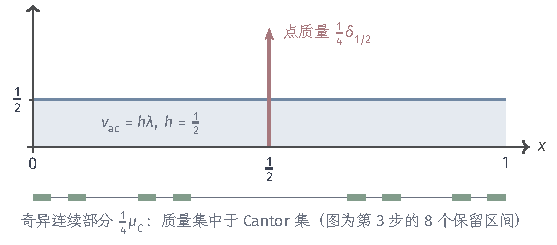
\includegraphics[width=94.365mm]{figures/02-abstract-mathematics/01-metric-and-measure/tikz/c4-lebesgue-density/figure.pdf}
  \caption{相对于长度测度的密度只表示绝对连续部分。$\rho=\tfrac12\lambda|_{[0,1]}+\tfrac14\delta_{1/2}+\tfrac14\mu_C$：蓝色区域是密度$h=1/2$表示的质量$1/2$；红色箭头是位于$1/2$的点质量$1/4$；下方绿色线段是Cantor集构造第$3$步保留的$8$个区间，Cantor测度的质量$1/4$集中在它们的极限——零长度的Cantor集上。后两部分都集中在长度零测集上，任何密度都无法表示。}
  \label{fig:dens-lebesgue-form}
\end{figure}

\paragraph{普通导数能恢复什么}
这个例子的累积函数在$[0,1]$上是$G(x)=\tfrac12x+\tfrac14\mathbf 1_{[1/2,\infty)}(x)+\tfrac14F_C(x)$。求它的普通导数：一次项的导数是$\tfrac12$；阶跃项在$x\neq1/2$处导数为零；Cantor函数在每个删去的开区间上为常数，而这些开区间的总长度为$1$，所以它几乎处处导数为零。于是$G'=\tfrac12$几乎处处，恰好是绝对连续部分的密度。

导数遗漏了另外两份质量：$\int_0^1G'\,\mathrm dx=\tfrac12$，而$G(1)-G(0)=1$，差额中$\tfrac14$是原点$1/2$处的跳跃，另$\tfrac14$是Cantor函数在零长度集合上的连续增长。这正是第~\ref{chap:integration}章所说的：连续性与几乎处处可导都不能保证函数由导数的积分恢复。一般地，实轴上有限Borel测度的累积函数几乎处处可导，导数几乎处处等于绝对连续部分的密度；这一结论属于Lebesgue微分定理，这里不给出证明。本章只在累积函数绝对连续时使用导数计算密度，见第~\ref{sec:dens-cumulative-density}小节。
